\chapter{Conclusion} \label{chap:con}

This thesis successfully addresses the challenge of automating a time-consuming manual process in the nuclear industry. Researchers are often required to perform repetitive, labor-intensive measurements. The primary goal was to develop a solution that integrates seamlessly into the researcher’s workflow without causing disruptions. The thesis focused on a specific category of coating-layer images with relatively homogeneous properties, in contrast to other types of images in the dataset. It was shown that segmentation of more complex, heterogeneous images is a viable direction for future work.

Three approaches were evaluated. First, the classical K-means algorithm was found to be computationally efficient, but it lacked universal applicability due to the variability of coating layers. This made it unsuitable for a streamlined workflow without extensive post-processing. Second, the Segment Anything Model (SAM) was considered, but hardware and precision limitations made it infeasible for the given problem. Finally, Convolutional Neural Networks (CNNs) were explored. This solution required labeled data. Three types of labels were developed. The model was trained on the most precise set, but it was found that even the least manually intensive labels were effective for training, although not as good as the most precise type.

The optimization and testing of the model were thoroughly discussed, with results measured using the Intersection over Union (IoU) metric alongside the Hausdorff distance. The model achieved a mean IoU of  95.155\%, demonstrating its high accuracy in segmenting coating layers.

The practical impact was clear after integrating the model into the researcher’s workflow. The time required for measurement tasks was reduced by half. For images similar to the training dataset, over 90\% of predicted measurements required no further manual adjustments. However, for images from sets with significantly different characteristics, performance declined, highlighting the need for further re-training.

With the code infrastructure in place, future improvements can focus on streamlining the training process and enhancing prediction accuracy. The current model was trained on fewer than 100 images from a limited number of sets, which is insufficient for creating a fully robust model. Nevertheless, even when incorrect, the model's average deviation was approximately five pixels, resulting in substantial time savings. This efficiency will accelerate the generation of additional labeled data, creating a feedback loop for continuous improvement. The iterative workflow is illustrated in Figure~\ref{fig:workflow-diagram}.

\begin{figure}[H]
    \centering
    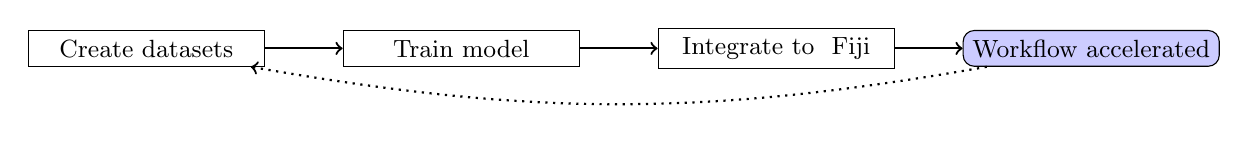
\begin{tikzpicture}[node distance=4cm, every node/.style={align=center, font=\small}, xscale=1]

        \node[rectangle, draw, minimum width=3cm] (dataset) {Create datasets};
        \node[rectangle, draw, minimum width=3cm, right of=dataset] (train) {Train model};
        \node[rectangle, draw, minimum width=3cm, right of=train] (integration) {Integrate to \ Fiji};
        \node[rectangle, draw, fill=blue!20, minimum width=3cm, right of=integration, rounded corners] (result) {Workflow accelerated};

        % Arrows
        \draw[->, thick] (dataset) -- (train);
        \draw[->, thick] (train) -- (integration);
        \draw[->, thick] (integration) -- (result);
        \draw[->, thick, dotted] (result) to[bend left=10] (dataset);
    \end{tikzpicture}
    \caption{Workflow of model integration and performance improvement.}
    \label{fig:workflow-diagram}
\end{figure}



%In conclusion, this thesis automates a portion of the researcher’s measurement process and establishes a pipeline for continuous model retraining and improvement. The improvements brought by this work will lead to time savings and improved efficiency. This work highlights the practical impact of deep learning in automating image analysis tasks in the nuclear industry.%


%Tohle mi trochu nesedí. Automatizace je dobrá a deep learning tomu umí pomoc. To víme. To co jsi udělala ty, je že jsi snížila "náklady" na aplikaci deep learningu tím, že jsi prozkoukamala klasické metody, které ti pomohou zrekonstruovat labely a ukázala, že jsou skutečně použitelné. To, že jsi nastartovala feedback loop z toho vyplývá.%
%Pokud bys tu měla něco změnit, tak je to tohle. Je důležité tu práci prodávat jako to co to je. Jinak by se mohlo zdát, že tvoje práce byla jenom aplikovat neuronky a to je pro akademiky triviální a nezajímavé. Ty jsi ale přišla s tím, jak překonat překážky vedoucí k aplikaci. %

In conclusion, this thesis automates a portion of the researcher’s measurement process by addressing the challenges of applying deep learning to image analysis tasks. By refining traditional methods for label reconstruction, this work establishes a cost-effective approach to preparing high-quality ground truth labels, enabling the successful application of deep learning. The improvements brought by this work will lead to significant time savings and enhanced efficiency, paving the way for continuous model retraining and further advancements.

\chapter{Appendix}

The complete implementation of this thesis, including preprocessing, label generation, model training, and evaluation scripts, is available at \href{https://github.com/emmateki/coating_detection}{GitHub} (\url{https://github.com/emmateki/coating_detection})


This project benefited from various open-source libraries that facilitated image processing, deep learning model training, and evaluation. A detailed list of dependencies and libraries used can be found in the repository’s environment file.
\chapter{Disclaimer}
I hereby declare that I have completed this thesis independently, with the assistance of artificial intelligence tools used for specific tasks throughout the writing process. I have thoroughly reviewed all AI-generated content to ensure its accuracy and correctness.

I take full responsibility for the information presented in this thesis, guaranteeing its reliability. The use of AI tools was conducted in compliance with ethical standards and academic integrity, ensuring that the work remains original and authentic.

The following tools were used, along with their respective purposes:

\begin{itemize}
    \item \textbf{Grammarly} (https://www.grammarly.com) - for text corrections
    \item \textbf{ChatGPT-4} (https://chat.openai.com/) - for rephrasing and text corrections
    \item \textbf{GitHub Copilot} (https://copilot.github.com) - for code corrections
\end{itemize}


